\documentclass{beamer}
%
% Choose how your presentation looks.
%
% For more themes, color themes and font themes, see:
% http://deic.uab.es/~iblanes/beamer_gallery/index_by_theme.html
%
\mode<presentation>
{
  \usetheme{Boadilla}      % or try Darmstadt, Madrid, Warsaw, ...
  \usecolortheme{beaver} % or try albatross, beaver, crane, ...
  \usefonttheme{default}  % or try serif, structurebold, ...
  \setbeamertemplate{navigation symbols}{}
  \setbeamertemplate{caption}[numbered]
  
} 

\usepackage{xcolor,colortbl}
\usepackage[english]{babel}
\usepackage[utf8x]{inputenc}
\usepackage{courier}
\usepackage{dsfont}
\usepackage{verbatim} 
\usepackage{enumerate}
\usepackage{tikz}
\usetikzlibrary{shapes.geometric, arrows}
\usepackage{multirow}
\usepackage{venndiagram}
\usepackage{epigraph} 
%\usepackage{xcolor}
\usepackage{makecell}

%\usepackage{enumitem}

\usepackage{hyperref}
\hypersetup{
    colorlinks=true,
    linkcolor=blue,
    filecolor=magenta,      
    urlcolor=cyan,
}

% R stuff!
\usepackage{listings}
\definecolor{codegreen}{rgb}{0,0.6,0}
\definecolor{codegray}{rgb}{0.5,0.5,0.5}
\definecolor{codepurple}{rgb}{0.58,0,0.82}
\definecolor{backcolour}{rgb}{0.95,0.95,0.92}

\lstdefinestyle{mystyle}{
    backgroundcolor=\color{backcolour},    
    commentstyle=\color{codegreen},
    keywordstyle=\color{black},
    numberstyle=\tiny\color{codegray},
    stringstyle=\color{codepurple},
    basicstyle=\ttfamily\footnotesize,
    breakatwhitespace=false,         
    breaklines=true,                 
    captionpos=b,                    
    keepspaces=true,                 
    numbers=left,                    
    numbersep=5pt,                  
    showspaces=false,                
    showstringspaces=false,
    showtabs=false,                  
    tabsize=2
}

\lstset{style=mystyle}


\setbeamertemplate{enumerate items}[default]
\setbeamertemplate{itemize item}[triangle]


\title[Introduction to Statistics]{Hypothesis Testing pt. 4}
\subtitle{More on Strength of Evidence and Test-stats}
\author{Grinnell College}
\date{}

\graphicspath{{img/}}

\begin{document}

\begin{frame}
  \titlepage
\end{frame}

\begin{frame}{Review}

Previously we introduced the idea of null distributions and test-statistics \\ \vspace{8mm}

If we were to collect many samples and compute $\overline{x}$, the null distribution refers to the distribution of statistics
\begin{align*}
t = \frac{\overline{x} - \mu_0}{\hat{\sigma}/\sqrt{n}}
\end{align*}
when $H_0:\mu = \mu_0$, i.e., the null hypothesis is true
\end{frame}

\begin{frame}{Test-Statistic}
\small
Consider the pieces of a t-statistic
\begin{align*}
T = \frac{\overline{x} - \mu_0}{\hat{\sigma}/\sqrt{n}}
\end{align*}
\begin{enumerate}
\item  $\overline{x} - \mu_0$ indicates the distance between my observed data and my null hypothesis, though we cannot use this alone as it does not include a degree of ``certainty" associated with $\overline{x}$
\item $\hat{\sigma}$ is my estimate of the population's standard deviation. When this is large, there will be more uncertainty in my estimate of $\overline{x}$
\item $n$ represents the number of observations in my sample -- the more observations I have, the more confidence I will have in my estimate 
\end{enumerate} \vspace{2mm}
We should have a sense of how each of these components impact my $t$-statistic
\end{frame}

\begin{frame}{Test-Statistic}
\begin{align*}
T = \frac{\overline{x} - \mu_0}{\hat{\sigma}/\sqrt{n}}
\end{align*}
We can think, then, of the t-statistic as being a measure of evidence \textit{against} the null hypothesis \\ \vspace{6mm}

If:
\begin{enumerate}
\item $\overline{x}$ is far from $\mu_0$ and
\item Our certainty in $\overline{x}$ is high (i.e., low $\hat{\sigma}$ or large $n$)
\end{enumerate}
then our statistic $T$ will be larger. \vspace{8mm}

A larger $T$ statistic is less likely than a smaller one when H$_0$ is true\\
\begin{itemize}
    \item What we consider ``large" will depend on the t-distribution
\end{itemize}
\end{frame}

\begin{frame}{t-distribution}
When the null hypothesis is true, 
\begin{align*}
t = \frac{\overline{x} - \mu_0}{\hat{\sigma}/\sqrt{n}}
\end{align*}
follows a $t$-distribution with $n-1$ degrees of freedom \\ \vspace{10mm}

The degrees of freedom tells us, relatively speaking, what values are considered ``large" \\ \vspace{4mm}

$T = 1.69$ may be considered ``large" when $df = 30$ but not when $df = 5$
\end{frame}

\begin{frame}{t-distribution Comparison}
\begin{center}
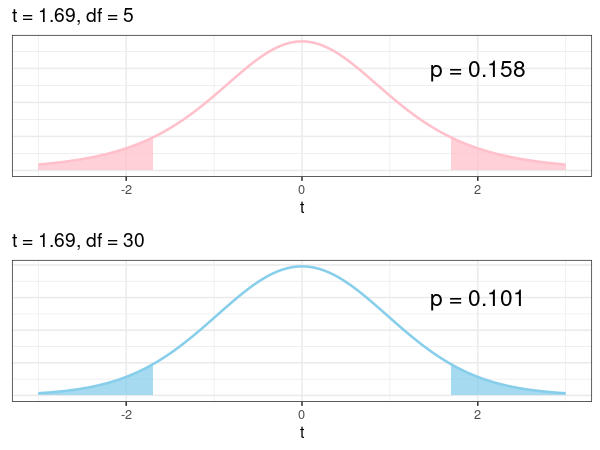
\includegraphics[scale=0.5]{img/pval_compare.png}
\end{center}
\end{frame}

\begin{frame}{Hypothesis Testing Summary}
The process goes like this:
\begin{enumerate}
\item Assume our null hypothesis $H_0:\mu = \mu_0$ is true
\item Compute a $T$-statistic with our observed data
\item Ask: is this $T$-statistic ``large"? 
\begin{itemize}
\item This will depend on the degrees of freedom
\end{itemize}
\item If we know our $T$ statistic and we know our degrees of freedom, we can find the probability of observing our data if the null is true. This probability is our \textbf{p-value}
\end{enumerate}
\end{frame}

\begin{frame}{P-values}
Hopefully by this point the utility of p-values is becoming clear
\begin{itemize}
    \item quantify how unlikely the data is \textit{if} H$_0$ is true
    \item take into account both the test-stat and the associated distribution
\end{itemize} \vspace{8mm}

When we say 'there is (evidence) against the null hypothesis', what we are doing is quantifying how far off the data is from what we would expect.
    
\end{frame}

\end{document}

